\subsection{Force validation}
\label{subsec:force_validation}

The last test that we will perform is the force validation.

Thanks to the data obtained from the previous tests, we should already be able to predict the force applied to the ball by the inductance.
In particular, we already know that the electromagnetic force applied to the ball is given by the following equation:

\begin{equation}
    F_{em} = \frac{1}{2} \frac{\partial L}{\partial z} I^2
\end{equation}

Because of the previously identified parameters, we have an analytical expression for the sensitivity of the inductance with respect to the position of the ball.
However, due to uncertainties in the identification of the parameters, we can expect some discrepancies between the predicted force and the measured one.

In order to quantify these discrepancies and validate the model, we will use a direct method to measure the force applied to the ball by the inductance and compare it with the predicted one.
To do so, we recall Equation \ref{eq:reduced_equations_of_motion_final} and in particular the equation relative to $\dot{v}$:

\begin{equation}
    \dot{v} = m^{-1} \left(\frac{1}{2} \frac{\partial L_1}{\partial z} I_1^2 + \frac{1}{2} \frac{\partial L_2}{\partial z} I_2^2 + m g  \right)
\end{equation}

If we consider the system at rest, we can simplify the equation as follows:

\begin{equation}
    0 = \frac{1}{2} \frac{\partial L_1}{\partial z} I_1^2 + \frac{1}{2} \frac{\partial L_2}{\partial z} I_2^2 + m g
\end{equation}

Supposing now that only the first coil is energized, we can further simplify the equation as follows:

\begin{equation}
    0 = \frac{1}{2} \frac{\partial L_1}{\partial z} I_1^2 + m g
\end{equation}

Which leads to:

\begin{equation}
    \frac{\partial L_1}{\partial z} = -2 \frac{m g}{I_1^2}
    \label{eq:sensitivity_of_inductance}
\end{equation}

This last equation basically tells us that in steady state conditions, when the ball is levitating (i.e. $\dot{z} = 0$ and not supported by any platform), the sensitivity of the inductance of the first coil has an analytical expression that can be directly measured by measuring the current in the first coil.

In order to follow this approach, a linearly increasing voltage has been applied to the first coil and the current corresponding to the levitation of the ball has been measured.
The test has been repeated for different initial positions of the ball, in order to fully characterize the dynamic inductance characteristics over the range of possible ball positions.

In Figure \ref{fig:levitation_current} we can see both the position of the ball and the current circulating in the first coil.
By identifying the current at which the ball starts to levitate (i.e. the ball starts to move upwards), we can than use Equation \ref{eq:sensitivity_of_inductance} to identify the dynamic inductance characteristics.

\begin{figure}[H]
    \centering
    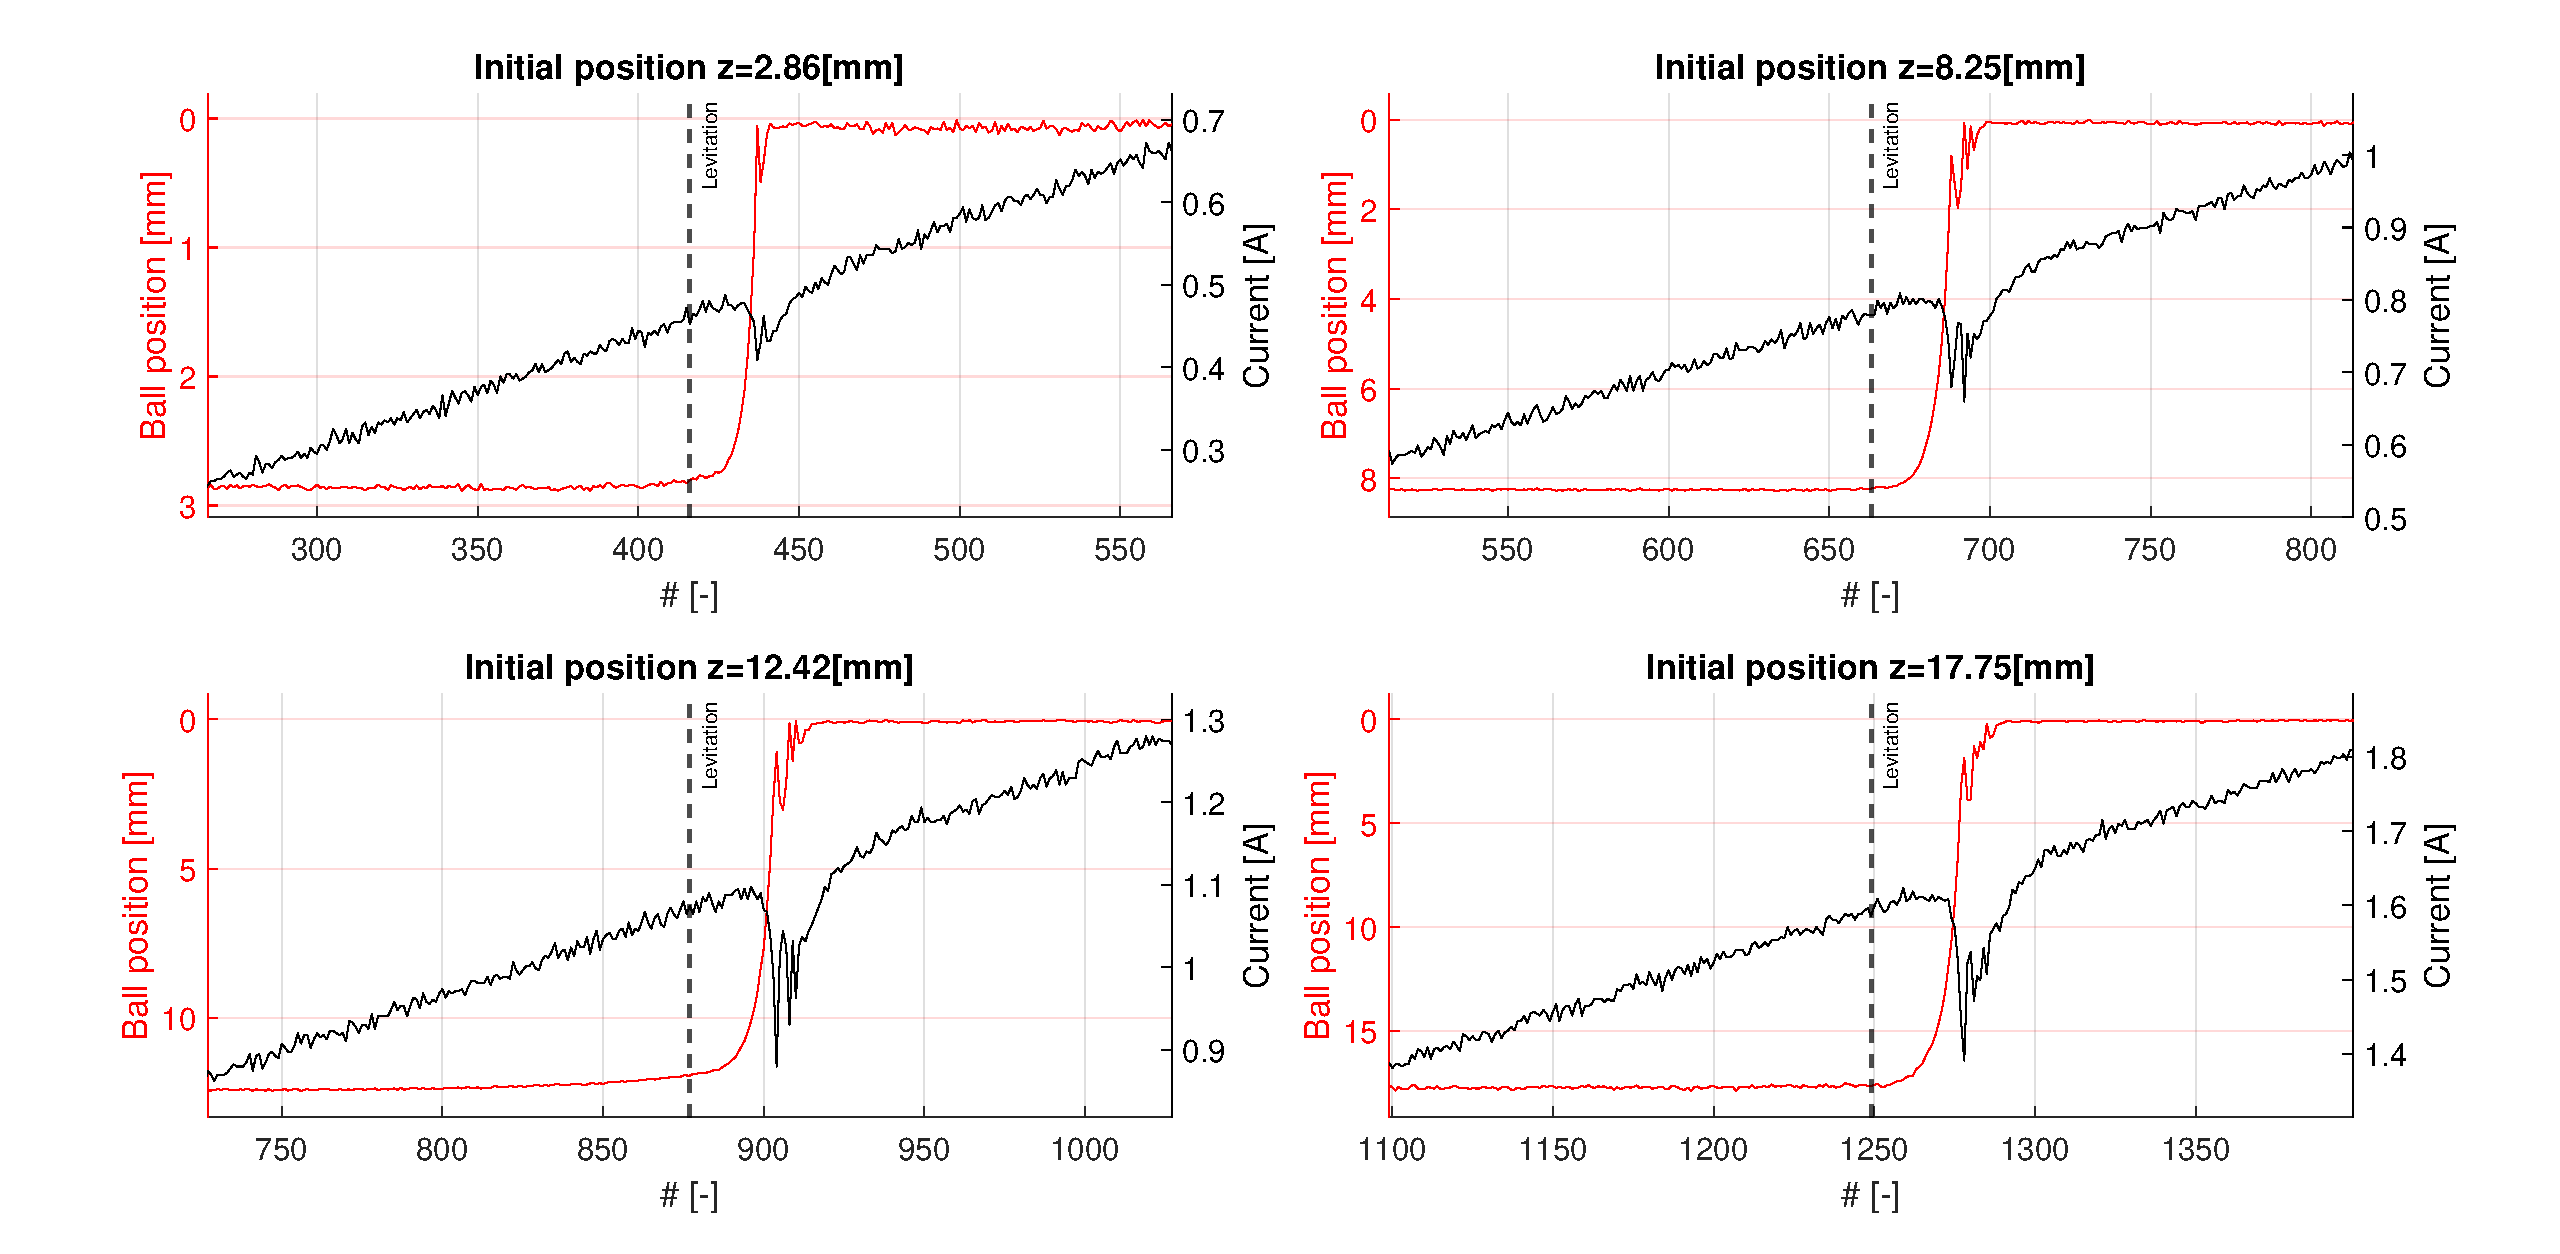
\includegraphics[width=1\textwidth]{img/MATLAB/identification/currents_for_force.pdf}
    \caption{Position of the ball and current in the first coil around the levitation point (marked by vertical black line)}
    \label{fig:levitation_current}
\end{figure}

In Figure \ref{fig:dynamic_inductance_characteristics}, we can observe both the measured data and the fitted ones.
On the right side figure, a complete characterization of the electromagnetic force has been reconstructed based again on the above equations.

\begin{figure}[H]
    \centering
    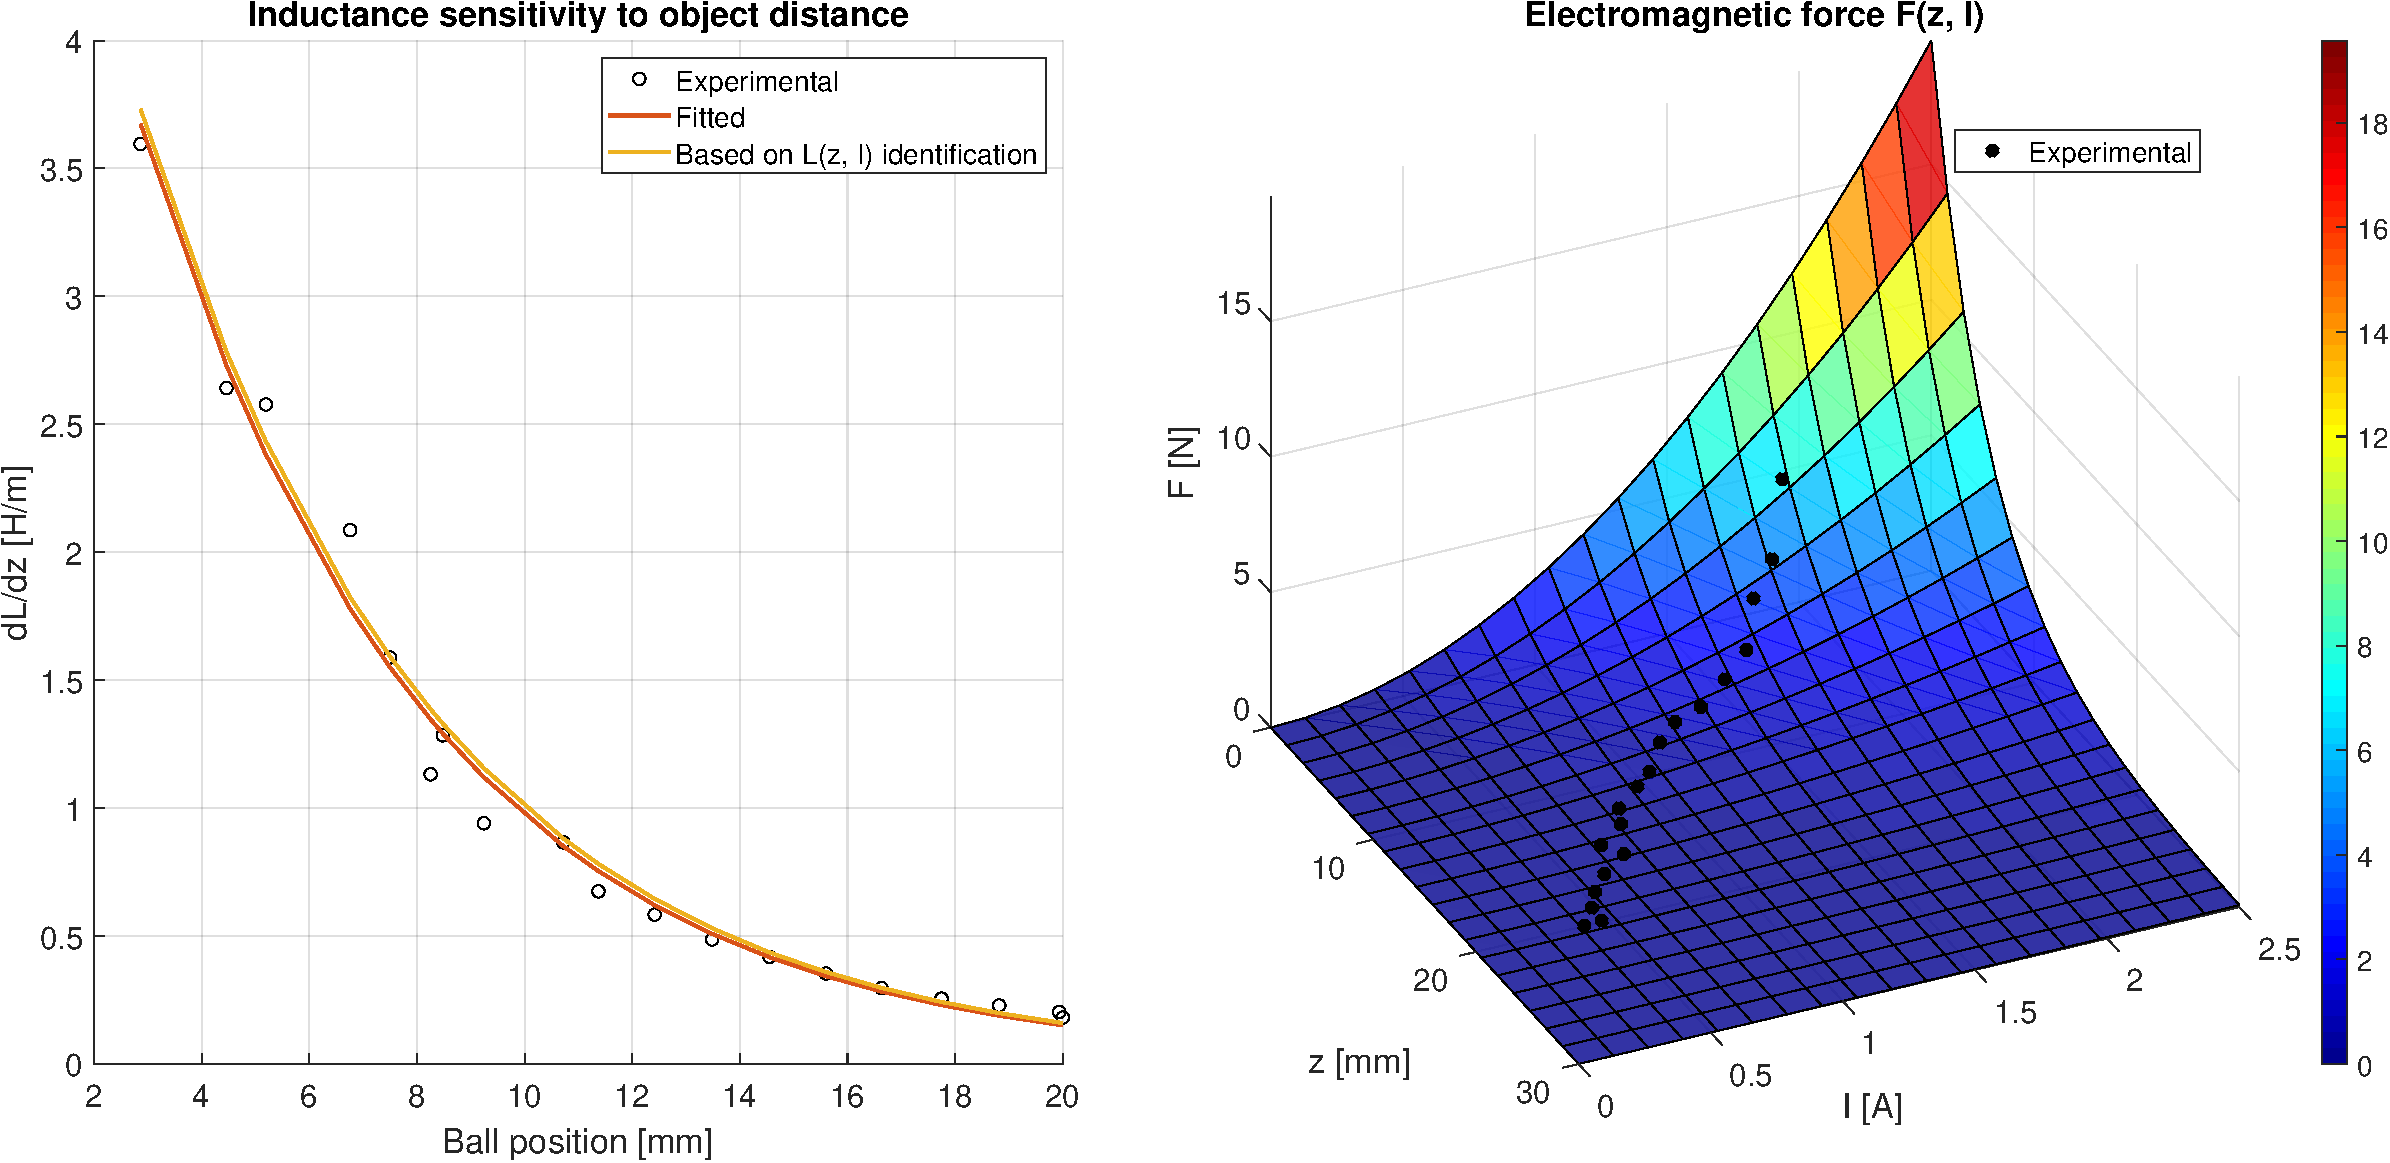
\includegraphics[width=1\textwidth]{img/MATLAB/identification/force.pdf}
    \caption{Dynamic inductance characteristics and electromagnet force}
    \label{fig:dynamic_inductance_characteristics}
\end{figure}

The left-hand side of Figure \ref{fig:dynamic_inductance_characteristics} shows a comparison between the measured data (black circles), their fitting (red line), the sensitivity of the inductance coming from the model (blue line) and the sensitivity of the inductance resulting from the literature parameters (green line).
Notice that the curve coming from the literature parameters has been doubled given the different model used for the electromagnetic force in the literature (see Equation \ref{eq:simplified_equations_of_motion_final}).

Data shows great accuracy in almost the entire range of the ball position, with a slight discrepancy in the lower part of the range.
This discrepancy is probably due to poor measurement quality because of high noise ratio given by the infrared sensor.

The right-hand side of Figure \ref{fig:dynamic_inductance_characteristics} shows the electromagnetic force generated by the first coil as a function of both the ball position and the current circulating in the coil.
One can notice that the force has an exponential behavior with respect to the ball position and a quadratic behavior with respect to the current.